\documentclass[11pt,a4paper]{report}
\usepackage[textwidth=37em,vmargin=30mm]{geometry}
\usepackage{calc,xunicode,amsmath,amssymb,paralist,enumitem,tabu,booktabs,datetime2,xeCJK,xeCJKfntef,listings}
\usepackage{tocloft,fancyhdr,tcolorbox,xcolor,graphicx,eso-pic,xltxtra,xelatexemoji}

\newcommand{\envyear}[0]{2025}
\newcommand{\envdatestr}[0]{2025-06-03}
\newcommand{\envfinaldir}[0]{webdb/2025/20250603/final}

\usepackage[hidelinks]{hyperref}
\hypersetup{
    colorlinks=false,
    pdfpagemode=FullScreen,
    pdftitle={Web Digest - \envdatestr}
}

\setlength{\cftbeforechapskip}{10pt}
\renewcommand{\cftchapfont}{\rmfamily\bfseries\large\raggedright}
\setlength{\cftbeforesecskip}{2pt}
\renewcommand{\cftsecfont}{\sffamily\small\raggedright}

\setdefaultleftmargin{2em}{2em}{1em}{1em}{1em}{1em}

\usepackage{xeCJK,xeCJKfntef}
\xeCJKsetup{PunctStyle=plain,RubberPunctSkip=false,CJKglue=\strut\hskip 0pt plus 0.1em minus 0.05em,CJKecglue=\strut\hskip 0.22em plus 0.2em}
\XeTeXlinebreaklocale "zh"
\XeTeXlinebreakskip = 0pt


\setmainfont{Brygada 1918}
\setromanfont{Brygada 1918}
\setsansfont{IBM Plex Sans}
\setmonofont{JetBrains Mono NL}
\setCJKmainfont{Noto Serif CJK SC}
\setCJKromanfont{Noto Serif CJK SC}
\setCJKsansfont{Noto Sans CJK SC}
\setCJKmonofont{Noto Sans CJK SC}

\setlength{\parindent}{0pt}
\setlength{\parskip}{8pt}
\linespread{1.15}

\lstset{
	basicstyle=\ttfamily\footnotesize,
	numbersep=5pt,
	backgroundcolor=\color{black!5},
	showspaces=false,
	showstringspaces=false,
	showtabs=false,
	tabsize=2,
	captionpos=b,
	breaklines=true,
	breakatwhitespace=true,
	breakautoindent=true,
	linewidth=\textwidth
}






\newcommand{\coverpic}[2]{
    % argv: itemurl, authorname
    Cover photo by #2~~(\href{#1}{#1})
}
\newcommand{\makeheader}[0]{
    \begin{titlepage}
        % \newgeometry{hmargin=15mm,tmargin=21mm,bmargin=12mm}
        \begin{center}
            
            \rmfamily\scshape
            \fontspec{BaskervilleF}
            \fontspec{Old Standard}
            \fontsize{59pt}{70pt}\selectfont
            WEB\hfill DIGEST
            
            \vfill
            % \vskip 30pt
            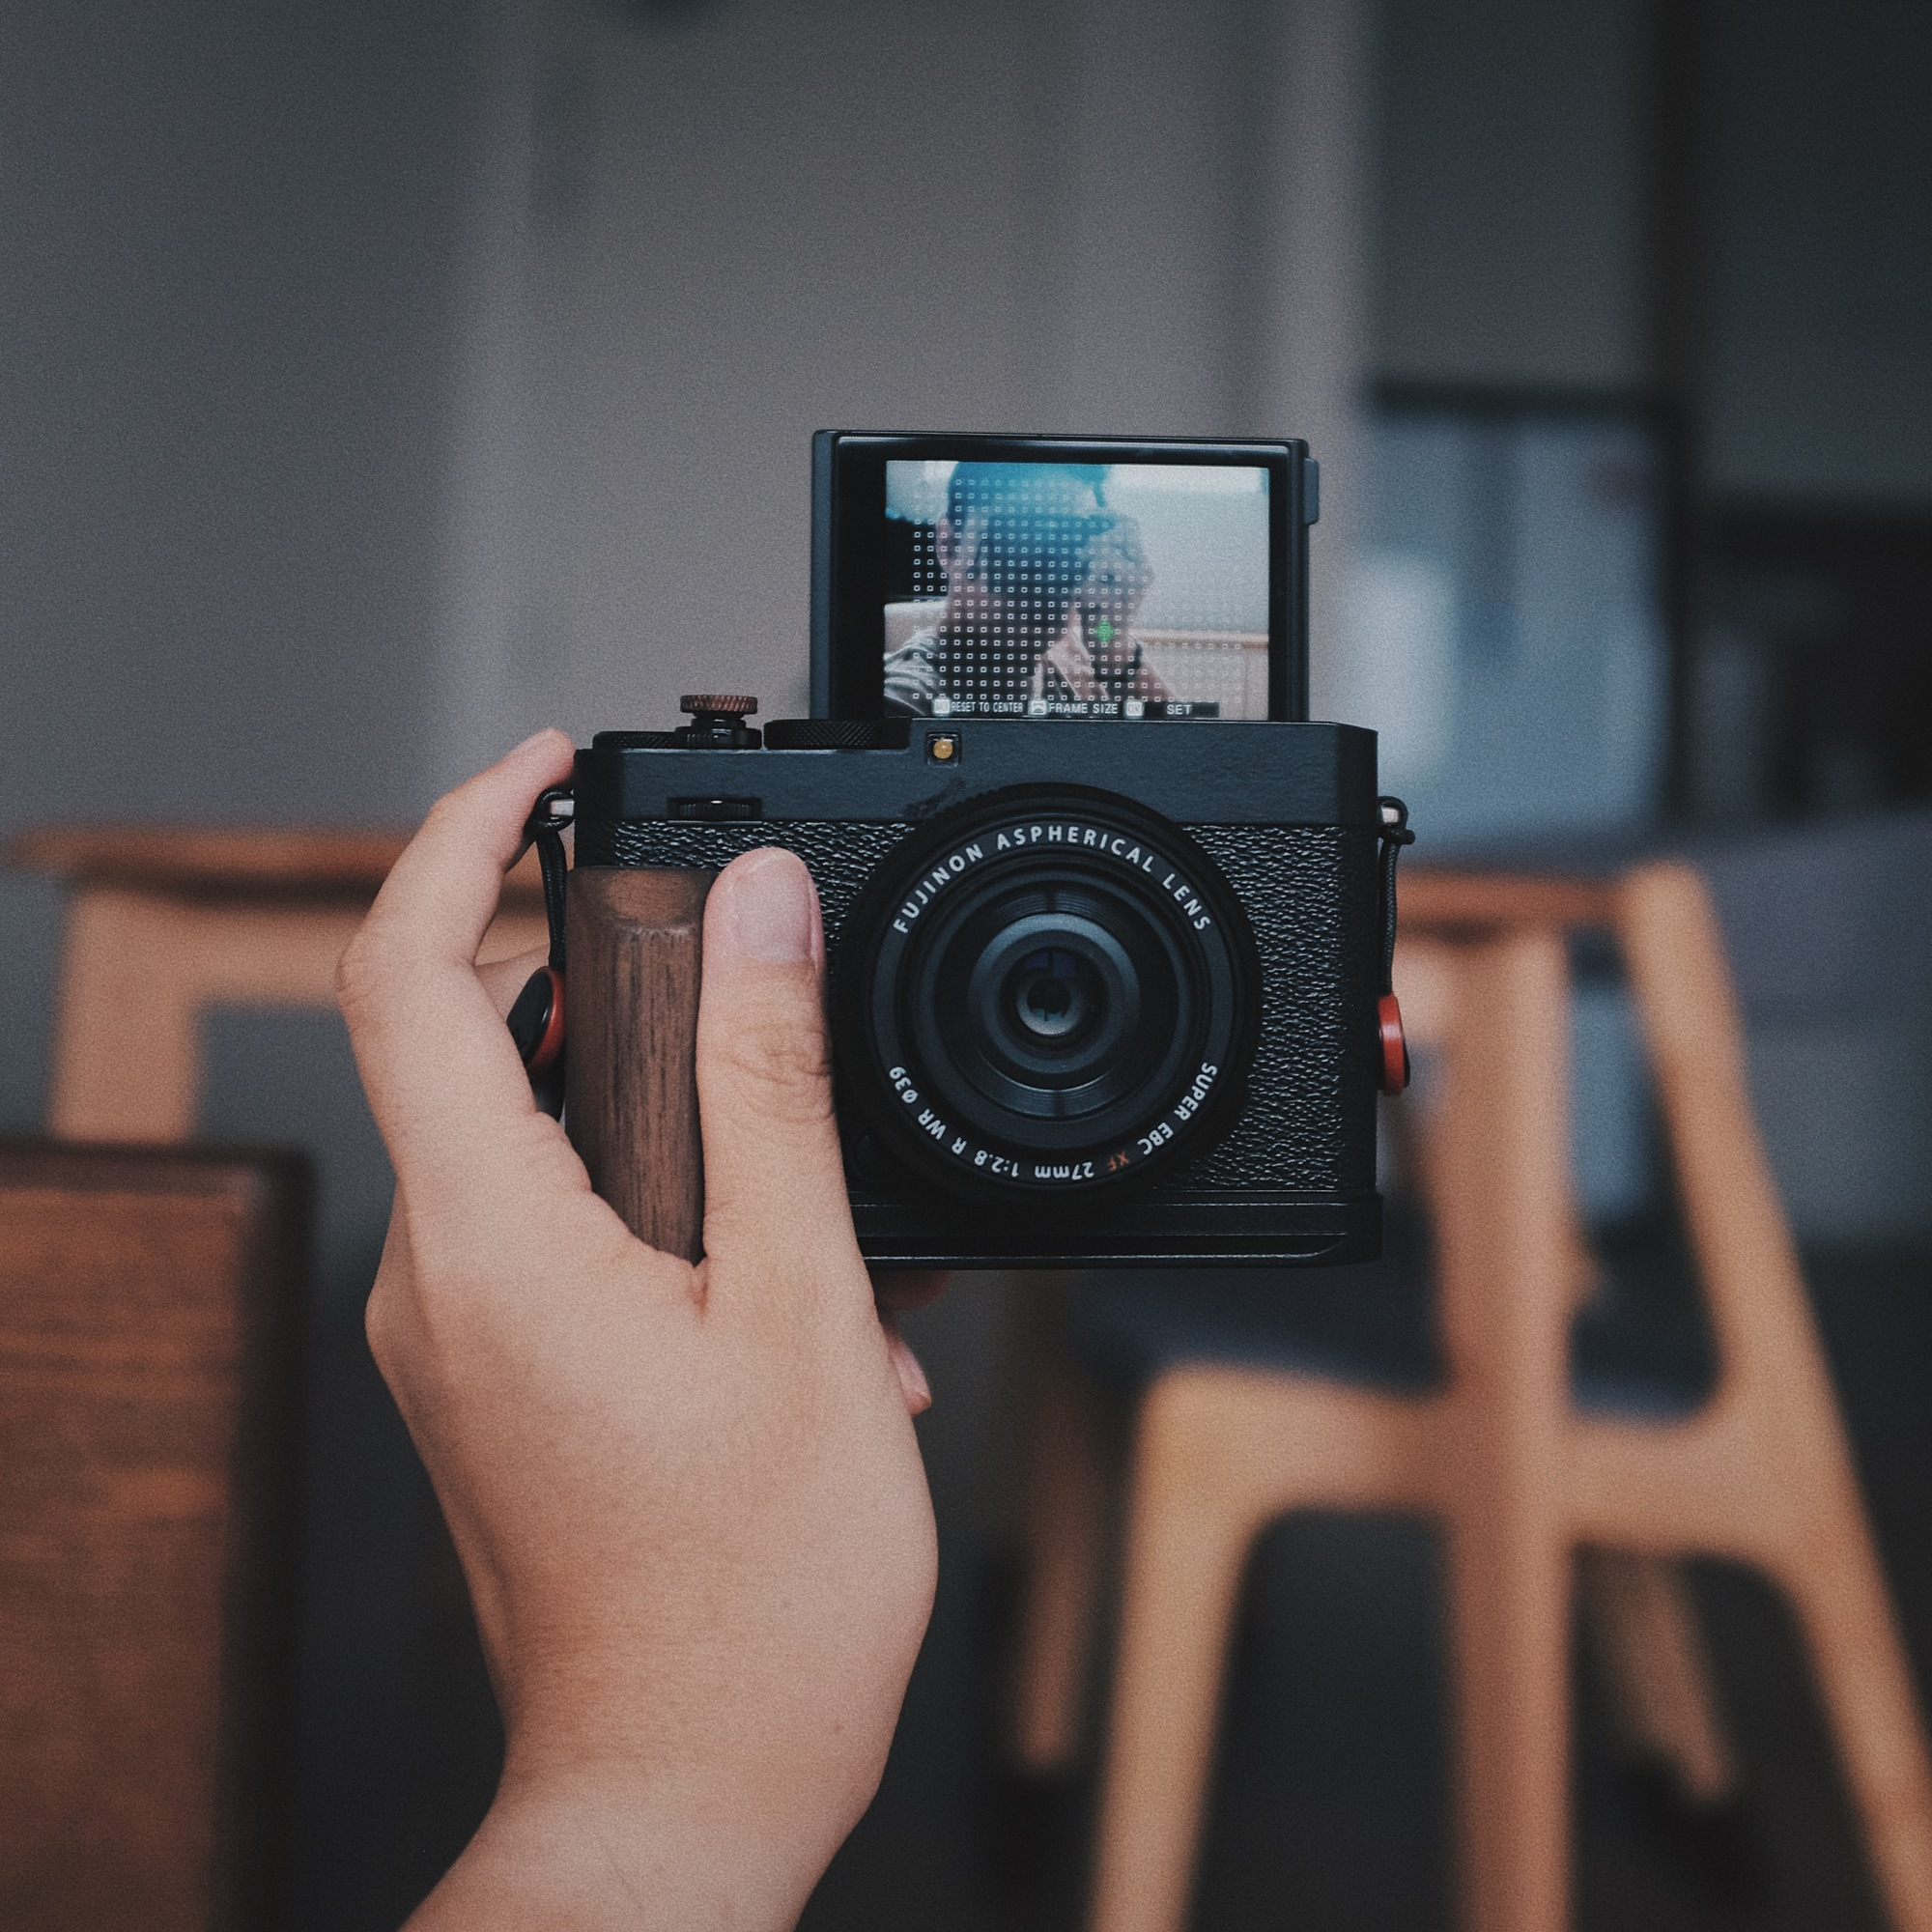
\includegraphics[width=\linewidth]{\envfinaldir/coverpic-prod.jpg}\par
            % \vskip 30pt
            \vfill

            \normalsize\rmfamily\scshape
            \copyright{} The Web Digest Project \hfill\large \envdatestr
        \end{center}
    \end{titlepage}
    % \restoregeometry
}
\newcommand{\simplehref}[1]{%
    \textcolor{blue!80!green}{\href{#1}{#1}}%
}
\renewcommand{\contentsname}{\center\Huge\sffamily\bfseries Contents\par\vskip 20pt}
\newcounter{ipartcounter}
\setcounter{ipartcounter}{0}
\newcommand{\ipart}[1]{
    % \vskip 20pt
    \clearpage
    \stepcounter{ipartcounter}
    \phantomsection
    \addcontentsline{toc}{chapter}{#1}
    % \begin{center}
    %     \Huge
    %     \sffamily\bfseries
    %     #1
    % \end{center}
    % \vskip 20pt plus 7pt
}
\newcounter{ichaptercounter}
\setcounter{ichaptercounter}{0}
\newcommand{\ichapter}[1]{
    % \vskip 20pt
    \clearpage
    \stepcounter{ichaptercounter}
    \phantomsection
    \addcontentsline{toc}{section}{\numberline{\arabic{ichaptercounter}}#1}
    \begin{center}
        \Huge
        \sffamily\bfseries
        #1
    \end{center}
    \vskip 20pt plus 7pt
}
\newcommand{\entrytitlefont}[1]{\subsection*{\raggedright\Large\sffamily\bfseries#1}}
\newcommand{\entryitemGeneric}[2]{
    % argv: title, url
    \parbox{\linewidth}{
        \entrytitlefont{#1}\par\vskip 5pt
        \footnotesize\ttfamily\mdseries
        \simplehref{#2}
    }\vskip 11pt plus 11pt minus 1pt
}
\newcommand{\entryitemGithub}[3]{
    % argv: title, url, desc
    \parbox{\linewidth}{
        \entrytitlefont{#1}\par\vskip 5pt
        \footnotesize\ttfamily\mdseries
        \simplehref{#2}\par\vskip 5pt
        \small\rmfamily\mdseries#3
    }\vskip 11pt plus 11pt minus 1pt
}
\newcommand{\entryitemAp}[3]{
    % argv: title, url, desc
    \parbox{\linewidth}{
        \entrytitlefont{#1}\par\vskip 5pt
        \footnotesize\ttfamily\mdseries
        \simplehref{#2}\par\vskip 5pt
        \small\rmfamily\mdseries#3
    }\vskip 11pt plus 11pt minus 1pt
}
\newcommand{\entryitemHackernews}[3]{
    % argv: title, hnurl, rawurl
    % \parbox{\linewidth}{
    %     \entrytitlefont{#1}\par\vskip 5pt
    %     \footnotesize\ttfamily\mdseries
    %     \simplehref{#3}\par
    %     \textcolor{black!50}{\href{#2}{#2}}
    % }\vskip 11pt plus 11pt minus 1pt
    \begin{minipage}{\linewidth}
            \entrytitlefont{#1}\par\vskip 5pt
            \footnotesize\ttfamily\mdseries
            \simplehref{#3}\par
            \textcolor{black!50}{\href{#2}{#2}}
    \end{minipage}\par\vskip 11pt plus 11pt minus 1pt
}







\begin{document}

\makeheader

\tableofcontents\clearpage




\ipart{Developers}
\ichapter{Hacker News}
\entryitemTwoLinks{My AI skeptic friends are all nuts}{https://news.ycombinator.com/item?id=44163063}{https://fly.io/blog/youre-all-nuts/}

\entryitemTwoLinks{The Unreliability of LLMs and What Lies Ahead}{https://news.ycombinator.com/item?id=44160573}{https://verissimo.substack.com/p/verissimo-monthly-may-2025}

\entryitemTwoLinks{Show HN: Penny-1.7B Irish Penny Journal style transfer}{https://news.ycombinator.com/item?id=44160073}{https://huggingface.co/dleemiller/Penny-1.7B}

\entryitemTwoLinks{Show HN: A toy version of Wireshark (student project)}{https://news.ycombinator.com/item?id=44159758}{https://github.com/lixiasky/vanta}

\entryitemTwoLinks{Ask HN: Who is hiring? (June 2025)}{https://news.ycombinator.com/item?id=44159528}{https://news.ycombinator.com/item?id=44159528}

\entryitemTwoLinks{Cloudlflare builds OAuth with Claude and publishes all the prompts}{https://news.ycombinator.com/item?id=44159166}{https://github.com/cloudflare/workers-oauth-provider/commits/main/}

\entryitemTwoLinks{Ask HN: How do I learn robotics in 2025?}{https://news.ycombinator.com/item?id=44158353}{https://news.ycombinator.com/item?id=44158353}

\entryitemTwoLinks{Whatever happened to cheap eReaders?}{https://news.ycombinator.com/item?id=44157701}{https://shkspr.mobi/blog/2025/05/whatever-happened-to-cheap-ereaders/}

\entryitemTwoLinks{TradeExpert, a trading framework that employs Mixture of Expert LLMs}{https://news.ycombinator.com/item?id=44157378}{https://arxiv.org/abs/2411.00782}

\entryitemTwoLinks{Show HN: Kan.bn – An open-source alterative to Trello}{https://news.ycombinator.com/item?id=44157177}{https://github.com/kanbn/kan}

\entryitemTwoLinks{If you are useful, it doesn't mean you are valued}{https://news.ycombinator.com/item?id=44156935}{https://betterthanrandom.substack.com/p/if-you-are-useful-it-doesnt-mean}

\entryitemTwoLinks{How reliable are MicroSD cards?}{https://news.ycombinator.com/item?id=44156142}{https://old.reddit.com/r/raspberry\_pi/comments/1l0v25s/how\_reliable\_are\_microsd\_cards\_well\_as\_it\_turns/}

\entryitemTwoLinks{How to post when no one is reading}{https://news.ycombinator.com/item?id=44155746}{https://www.jeetmehta.com/posts/thrive-in-obscurity}

\entryitemTwoLinks{The Princeton INTERCAL Compiler's source code}{https://news.ycombinator.com/item?id=44155247}{https://esoteric.codes/blog/published-for-the-first-time-the-original-intercal72-compiler-code}

\entryitemTwoLinks{The Visual World of 'Samurai Jack'}{https://news.ycombinator.com/item?id=44154032}{https://animationobsessive.substack.com/p/the-visual-world-of-samurai-jack}

\entryitemTwoLinks{LibriVox}{https://news.ycombinator.com/item?id=44153738}{https://librivox.org/}

\entryitemTwoLinks{The rise of judgement over technical skill}{https://news.ycombinator.com/item?id=44153732}{https://notsocommonthoughts.com/blog/ai-and-judgement/}

\entryitemTwoLinks{M8.2 solar flare, Strong G4 geomagnetic storm watch}{https://news.ycombinator.com/item?id=44152154}{https://www.spaceweatherlive.com/en/news/view/581/20250531-m8-2-solar-flare-strong-g4-geomagnetic-storm-watch.html}

\entryitemTwoLinks{Root shell on a credit card terminal}{https://news.ycombinator.com/item?id=44150803}{https://stefan-gloor.ch/yomani-hack}

\entryitemTwoLinks{Ukraine destroys more than 40 military aircraft in drone attack deep in Russia}{https://news.ycombinator.com/item?id=44150789}{https://www.npr.org/2025/06/01/nx-s1-5419509/ukraine-destroys-military-aircraft-attack-inside-russia-planes}\ichapter{Phoronix}
\entryitemGeneric{\hskip 0pt{}More Intel Panther Lake Graphics Device IDs Added To Open-Source Linux Driver}{https://www.phoronix.com/news/More-PTL-DIDs-Mesa-25.2}

\entryitemGeneric{\hskip 0pt{}Kexec HandOver "KHO" Merged For Linux 6.16}{https://www.phoronix.com/news/Kexec-HandOver-KHO-In-Linux-616}

\entryitemGeneric{\hskip 0pt{}Open-Source TPDE Can Compile Code 10-20x Faster Than LLVM}{https://www.phoronix.com/news/TPDE-Faster-Compile-Than-LLVM}

\entryitemGeneric{\hskip 0pt{}Linux 6.16 Will Now Conveniently Report Hard/Soft Lockups \& RCU Stall Counts}{https://www.phoronix.com/news/Linux-6.16-Hard-Soft-Lockups}

\entryitemGeneric{\hskip 0pt{}Power \& Performance Tuning For The Framework 13 With AMD Ryzen AI 300 Series}{https://www.phoronix.com/review/framework-13-ryzen-ai-power}

\entryitemGeneric{\hskip 0pt{}Phoronix Turns 21 This Week - Show Your Support For Linux Hardware Reviews}{https://www.phoronix.com/news/Phoronix-21-Birthday-Premium}

\entryitemGeneric{\hskip 0pt{}NFS Server Supporting Larger I/O Block Size With Linux 6.16}{https://www.phoronix.com/news/Linux-6.16-NFSD}

\entryitemGeneric{\hskip 0pt{}Mesa 25.2 Lands RADV VCN5 Video Encode/Decode Support For RDNA4 GPUs}{https://www.phoronix.com/news/Mesa-25.2-VCN5-RDNA4-Video}

\entryitemGeneric{\hskip 0pt{}Intel TDX Host Support Merged For KVM With Linux 6.16}{https://www.phoronix.com/news/Intel-TDX-Host-KVM-Linux-6.16}\ichapter{Dribbble}
\entryitemGeneric{\hskip 0pt{}Mnp Technologies - Logo Design}{https://dribbble.com/shots/26092034-Mnp-Technologies-Logo-Design}

\entryitemGeneric{\hskip 0pt{}Singular Logo Concept (Unused)}{https://dribbble.com/shots/26091755-Singular-Logo-Concept-Unused}

\entryitemGeneric{\hskip 0pt{}Cre8tera // Website}{https://dribbble.com/shots/26091009-Cre8tera-Website}

\entryitemGeneric{\hskip 0pt{}zeero logo design}{https://dribbble.com/shots/26087342-zeero-logo-design}

\entryitemGeneric{\hskip 0pt{}Shori Brand}{https://dribbble.com/shots/26088139-Shori-Brand}

\entryitemGeneric{\hskip 0pt{}Create email inbox composition}{https://dribbble.com/shots/26083118-Create-email-inbox-composition}

\entryitemGeneric{\hskip 0pt{}Roaring Bear}{https://dribbble.com/shots/26087788-Roaring-Bear}

\entryitemGeneric{\hskip 0pt{}Eagle}{https://dribbble.com/shots/26085536-Eagle}

\entryitemGeneric{\hskip 0pt{}Dog Mascot Various Poses}{https://dribbble.com/shots/26087977-Dog-Mascot-Various-Poses}

\entryitemGeneric{\hskip 0pt{}Hand-drawn illustration pack}{https://dribbble.com/shots/26084735-Hand-drawn-illustration-pack}

\entryitemGeneric{\hskip 0pt{}Branding Concept for Europe}{https://dribbble.com/shots/26087652-Branding-Concept-for-Europe}

\entryitemGeneric{\hskip 0pt{}B2B Dashboard \& Web App UI UX Design for Carbon Solutions}{https://dribbble.com/shots/26076624-B2B-Dashboard-Web-App-UI-UX-Design-for-Carbon-Solutions}

\entryitemGeneric{\hskip 0pt{}Patriot Logo Design (Unused for Sale)}{https://dribbble.com/shots/26081047-Patriot-Logo-Design-Unused-for-Sale}

\entryitemGeneric{\hskip 0pt{}Apple}{https://dribbble.com/shots/26084067-Apple}

\entryitemGeneric{\hskip 0pt{}Heliopoint}{https://dribbble.com/shots/26081987-Heliopoint}

\entryitemGeneric{\hskip 0pt{}Illustration}{https://dribbble.com/shots/26083223-Illustration}

\entryitemGeneric{\hskip 0pt{}Europe Logo Animation}{https://dribbble.com/shots/26082596-Europe-Logo-Animation}

\entryitemGeneric{\hskip 0pt{}Arc Logo}{https://dribbble.com/shots/26083648-Arc-Logo}

\entryitemGeneric{\hskip 0pt{}Heyo Turns 2!}{https://dribbble.com/shots/26078572-Heyo-Turns-2}

\entryitemGeneric{\hskip 0pt{}Roaring Bear}{https://dribbble.com/shots/26077332-Roaring-Bear}

\entryitemGeneric{\hskip 0pt{}Smart Home App}{https://dribbble.com/shots/26076565-Smart-Home-App}

\entryitemGeneric{\hskip 0pt{}Fox Brand Mascot}{https://dribbble.com/shots/26077954-Fox-Brand-Mascot}

\entryitemGeneric{\hskip 0pt{}Europe Logo Concept}{https://dribbble.com/shots/26077297-Europe-Logo-Concept}

\entryitemGeneric{\hskip 0pt{}Game Studio Logo}{https://dribbble.com/shots/26076821-Game-Studio-Logo}


\ipart{Developers~~~~(zh-Hans)}
\ichapter{Solidot}
\entryitemGeneric{\hskip 0pt{}美国的加密货币战略储备规模有多大}{https://www.solidot.org/story?sid=81446}

\entryitemGeneric{\hskip 0pt{}俄罗斯公共采购数据库泄漏核基地细节}{https://www.solidot.org/story?sid=81445}

\entryitemGeneric{\hskip 0pt{}黑猩猩将敲击树干作为一种交流模式}{https://www.solidot.org/story?sid=81444}

\entryitemGeneric{\hskip 0pt{}美国科技公司减少招聘应届生}{https://www.solidot.org/story?sid=81443}

\entryitemGeneric{\hskip 0pt{}AI 耗电量预计将在年底超过比特币}{https://www.solidot.org/story?sid=81442}

\entryitemGeneric{\hskip 0pt{}NASA 卫星确认火星溅射的证据}{https://www.solidot.org/story?sid=81441}

\entryitemGeneric{\hskip 0pt{}世界面临新形式的气候否认——经济不可行}{https://www.solidot.org/story?sid=81440}

\entryitemGeneric{\hskip 0pt{}越来越多的中国游戏公司开发单机游戏}{https://www.solidot.org/story?sid=81439}

\entryitemGeneric{\hskip 0pt{}天文学家发现以 44 分钟周期发射无线电波和 X 射线的神秘天体}{https://www.solidot.org/story?sid=81438}\ichapter{V2EX}
\entryitemGeneric{\hskip 0pt{}[问与答] 为什么水深火热节点突然访问不了了}{https://www.v2ex.com/t/1135902}

\entryitemGeneric{\hskip 0pt{}[酷工作] 支付相关远程资深前端开发,工资可以周结}{https://www.v2ex.com/t/1135901}

\entryitemGeneric{\hskip 0pt{}[问与答] 华硕路由器升级以后,智能家电无法连入、控制。}{https://www.v2ex.com/t/1135900}

\entryitemGeneric{\hskip 0pt{}[职场话题] 深圳房产中介,能干一辈子不?}{https://www.v2ex.com/t/1135899}

\entryitemGeneric{\hskip 0pt{}[酷工作] 找一个 UI 兼职。}{https://www.v2ex.com/t/1135897}

\entryitemGeneric{\hskip 0pt{}[推广] imgbed.cn 被我捡起来了}{https://www.v2ex.com/t/1135896}

\entryitemGeneric{\hskip 0pt{}[酷工作] [全球远程] Airbnb China 招各个级别的 Backend Engineers}{https://www.v2ex.com/t/1135895}

\entryitemGeneric{\hskip 0pt{}[程序员] 告别繁琐的滚动: Prompt Navigator 让 AI 对话历史回溯更轻松}{https://www.v2ex.com/t/1135893}

\entryitemGeneric{\hskip 0pt{}[问与答] 求问安卓上好用的图库和记账 APP}{https://www.v2ex.com/t/1135892}

\entryitemGeneric{\hskip 0pt{}[问与答] 工行的待遇真的非常差吗,应该是柜员岗,镇区分行}{https://www.v2ex.com/t/1135890}

\entryitemGeneric{\hskip 0pt{}[问与答] 淘宝无法使用消费券怎么个事啊?}{https://www.v2ex.com/t/1135889}

\entryitemGeneric{\hskip 0pt{}[生活] 如何匿名向 12315, 12345, 12320 举报?}{https://www.v2ex.com/t/1135885}

\entryitemGeneric{\hskip 0pt{}[问与答] celery 零停机部署有什么好方法吗?}{https://www.v2ex.com/t/1135884}

\entryitemGeneric{\hskip 0pt{}[推广] ChatGPT-4o GPT-4.1/Claude Sonnet 4/DeepSeek/Gemini 2.5 平台}{https://www.v2ex.com/t/1135882}

\entryitemGeneric{\hskip 0pt{}[视频技术] DJI Action 被自动分段的视频如何无痕拼接}{https://www.v2ex.com/t/1135881}

\entryitemGeneric{\hskip 0pt{}[推广] 又更新了一版我的网站}{https://www.v2ex.com/t/1135880}

\entryitemGeneric{\hskip 0pt{}[买买买] 有点闲钱,想花钱买快乐,求老哥们推荐,预算 6 万}{https://www.v2ex.com/t/1135879}

\entryitemGeneric{\hskip 0pt{}[宽带症候群] 广州商业地址,装什么宽带好一点。}{https://www.v2ex.com/t/1135878}

\entryitemGeneric{\hskip 0pt{}[Linux] Gnome 窗口 变得不可以点击,折磨了我一个假期啊!}{https://www.v2ex.com/t/1135877}

\entryitemGeneric{\hskip 0pt{}[问与答] windows 上 chrome 降级好像必须先卸载新版本才行?}{https://www.v2ex.com/t/1135876}

\entryitemGeneric{\hskip 0pt{}[写周报] 独立开发周记 120:靠苹果赚的钱都得还回去}{https://www.v2ex.com/t/1135875}

\entryitemGeneric{\hskip 0pt{}[知乎] 为什么知乎总是在推荐里推荐很多看过的内容}{https://www.v2ex.com/t/1135873}

\entryitemGeneric{\hskip 0pt{}[VXNA] 申请收录博客:地球人的空间}{https://www.v2ex.com/t/1135872}

\entryitemGeneric{\hskip 0pt{}[分享发现] 中国移动网龄回馈能薅羊毛了}{https://www.v2ex.com/t/1135871}

\entryitemGeneric{\hskip 0pt{}[宽带症候群] 广州珠村. 有没有佬有便宜宽带推荐下.}{https://www.v2ex.com/t/1135869}

\entryitemGeneric{\hskip 0pt{}[分享创造] Everlyn.app | 嫌 AI 生视频太慢,搞了个 15s 快速生成 5s 视频的工具,附带搞了个全免费、无限制的 AI 图像生成器}{https://www.v2ex.com/t/1135868}

\entryitemGeneric{\hskip 0pt{}[职场话题] 求深圳社平工资官方数据}{https://www.v2ex.com/t/1135867}

\entryitemGeneric{\hskip 0pt{}[问与答] Certbot Nginx OSCP 的正确打开方式是什么}{https://www.v2ex.com/t/1135866}

\entryitemGeneric{\hskip 0pt{}[远程工作] \# 人像图像篡改检测算法及软件开发(兼职)}{https://www.v2ex.com/t/1135865}

\entryitemGeneric{\hskip 0pt{}[生活] 温馨提示:网购玩具枪无法退货}{https://www.v2ex.com/t/1135862}

\entryitemGeneric{\hskip 0pt{}[职场话题] 这样算顶撞领导吗?}{https://www.v2ex.com/t/1135861}

\entryitemGeneric{\hskip 0pt{}[软件] 扫描文档 App 有什么推荐吗?}{https://www.v2ex.com/t/1135859}

\entryitemGeneric{\hskip 0pt{}[云计算] 为什么云是做电商的 Amazon 先搞出来,行业标准也是 AWS 的?为什么不是更有技术含量的 Microsoft、Google 先搞出来?}{https://www.v2ex.com/t/1135858}

\entryitemGeneric{\hskip 0pt{}[程序员] 租服务器部署满血版 deepseek 大概要多少钱}{https://www.v2ex.com/t/1135857}

\entryitemGeneric{\hskip 0pt{}[投资] 炒股做笔记真的有意义吗?}{https://www.v2ex.com/t/1135856}

\entryitemGeneric{\hskip 0pt{}[IPv6] ipv6 是不是会影响抖音和 bilibili}{https://www.v2ex.com/t/1135855}

\entryitemGeneric{\hskip 0pt{}[V2EX API] https://www.v2ex.com/api/v2/topics/1/replies?p=2 接口分页参数无效}{https://www.v2ex.com/t/1135854}

\entryitemGeneric{\hskip 0pt{}[NAS] 飞牛云 APP 在开启圈 X 的情况下没办法访问自己下载的应用,显示一片空白}{https://www.v2ex.com/t/1135852}

\entryitemGeneric{\hskip 0pt{}[奇思妙想] 有人会用番茄工作法吗?我想做一个``番茄搭子''AI,不知道大家会希望它怎么陪你?}{https://www.v2ex.com/t/1135851}

\entryitemGeneric{\hskip 0pt{}[分享发现] 必应壁纸自动安装原神}{https://www.v2ex.com/t/1135850}

\entryitemGeneric{\hskip 0pt{}[问与答] 现在还有必要充迅雷会员么?}{https://www.v2ex.com/t/1135849}

\entryitemGeneric{\hskip 0pt{}[NAS] 除了 synology drive,还有支持选择性同步的本地部署云盘吗}{https://www.v2ex.com/t/1135848}

\entryitemGeneric{\hskip 0pt{}[问与答] 有人想跑滴滴不?跑了 5 个小时狂赚 ¥73.1 元!}{https://www.v2ex.com/t/1135846}

\entryitemGeneric{\hskip 0pt{}[问与答] 推特号突然没了还能申诉回来么?}{https://www.v2ex.com/t/1135845}

\entryitemGeneric{\hskip 0pt{}[问与答] 笔记类应用数量这么多,为什么总是感觉满足不了自己的需求?}{https://www.v2ex.com/t/1135842}

\entryitemGeneric{\hskip 0pt{}[问与答] 显示器选择 EW3270U 和某🐟杂牌显示器}{https://www.v2ex.com/t/1135841}

\entryitemGeneric{\hskip 0pt{}[酷工作] Hot/New Jobs: Quant traders、DeFi trader、Quant engineer / developper 高级低延迟量化交易开发工程师 大数据开发工程师 DevOps 工程师}{https://www.v2ex.com/t/1135838}

\entryitemGeneric{\hskip 0pt{}[职场话题] 四线城市高校教师一辈子能有多少收入和存款}{https://www.v2ex.com/t/1135835}

\entryitemGeneric{\hskip 0pt{}[分享创造] 在四川,每个人都有个亲戚是开麻将馆的。}{https://www.v2ex.com/t/1135833}


\ipart{Generic News}







\clearpage
\leavevmode\vfill
\footnotesize

Copyright \copyright{} 2023-2025 Neruthes and other contributors.

This document is published with CC BY-NC-ND 4.0 license.

The entries listed in this newsletter may be copyrighted by their respective creators.

This newsletter is generated by the Web Digest project.

The newsletters are also delivered via Telegram channel \CJKunderline{\href{https://t.me/webdigestchannel}{https://t.me/webdigestchannel}}.\\
RSS feed is available at \CJKunderline{\href{https://webdigest.pages.dev/rss.xml}{https://webdigest.pages.dev/rss.xml}}.

This newsletter is available in PDF at
\CJKunderline{\href{https://webdigest.pages.dev/}{https://webdigest.pages.dev/}}.

The source code being used to generate this newsletter is available at\\
\CJKunderline{\href{https://github.com/neruthes/webdigest}{https://github.com/neruthes/webdigest}}.

This newsletter is also available in
\CJKunderline{\href{http://webdigest.pages.dev/readhtml/\envyear/WebDigest-20250603.html}{HTML}} and
\CJKunderline{\href{https://github.com/neruthes/webdigest/blob/master/markdown/\envyear/WebDigest-20250603.md}{Markdown}}.


\coverpic{https://unsplash.com/photos/woman-smiles-and-poses-in-a-field-at-sunset-0aSK030A69c}{Karsten Winegeart}


\end{document}
